\documentclass[a4paper,11pt, twocolumn]{article}
\usepackage[margin=0.8in]{geometry}
\usepackage{xcolor}
\usepackage{graphicx} %package to manage images
\graphicspath{ {./images/} }

\title{A2-04 Wireless Transmission}
\author{Revision sheet}
\date{}

\usepackage{fancyhdr}
\pagestyle{fancy}
\fancyhead{} % clear all header fields
\renewcommand{\headrulewidth}{0pt} % no line in header area
\fancyfoot{} % clear all footer fields
\renewcommand{\footrulewidth}{0.4pt}
\fancyfoot[C]{\thepage} % page number in centre of the page
\fancyfoot[R]{\footnotesize Thomas Boxall \\ Images from WJEC E-Book} % right hand footer has author name on top line and images reference on bottom line
\fancyfoot[L]{\footnotesize A2-04 Wireless Transmission \\ Revision sheet} % left hand footer has title of document on top line and 'Revision Sheet' on bottom line


\begin{document}

\maketitle
\thispagestyle{fancy}

% CONTENTS OF THE REVISION SHEET HERE
\section{Waves}
\subsection{Wavelength}
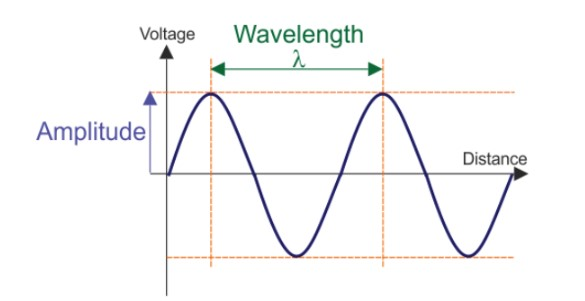
\includegraphics[width=0.45\textwidth]{wavelength.jpg}\\
Wavelength is a measure of distance between two adjacent points in a repeating wave. It is measured in meters ($m$).
\subsection{Wave Speed}
Wave speed ($c$) is how fast the wave propagates, this is usually the speed of light which is $3\times 10^8 ms^{-1}$. Frequency ($f$) gives number of cycles per second, usually in hertz. Wavelength ($\lambda$) gives distance of one cycle, usually in meters. These three factors can be combined to make the following equation.\\
$\displaystyle c =  f \lambda $
\subsection{Types Of Waves}
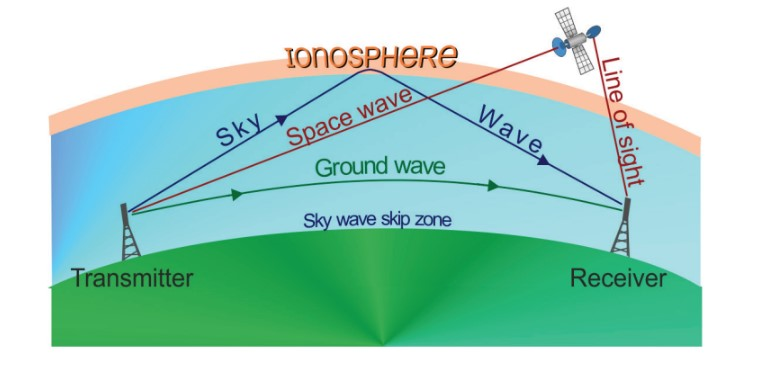
\includegraphics[width=0.45\textwidth]{typesOfWaves.jpg}\\
\subsubsection{Ground Waves}
These occur at frequencies below $3MHz$, follow the curvature of the earth and can travel 1000s of miles.
\subsubsection{Sky Waves}
These occur at $3$ to $30MHz$, go up into the sky, bounce off the ionosphere and come back down, can travel a very long distance and has a skip zone (this doesn't get any of the signal).
\subsubsection{Line-Of-Sight Waves}
These occur at frequencies above $30MHz$ and the transmitters are often built on hills as you need line of sight from the transmitter to the receiver.
\subsubsection{Space Waves}
These occur at $1$ to $300GHz$. 

\section{AM Radio}
In \textit{Amplitude Modulated} radio, the signal consists of two elements - a high frequency carrier wave and the information signal.\\
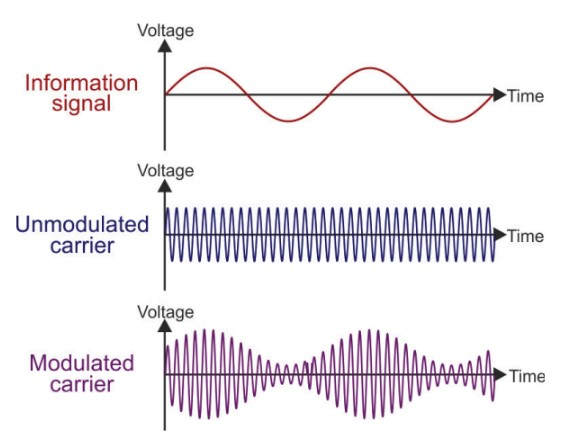
\includegraphics[width=0.45\textwidth]{amWave.jpg}\\
The information signal ($f_i$) is modulated onto the carrier signal ($f_c$). 
The AM modulated signal has the same frequency as the carrier wave. 
\subsection{Frequency Spectrum}
\subsubsection{Sine Waves}
A pure sinusoidal wave modulated onto a carrier frequency will produce the following frequency spectrum.\\
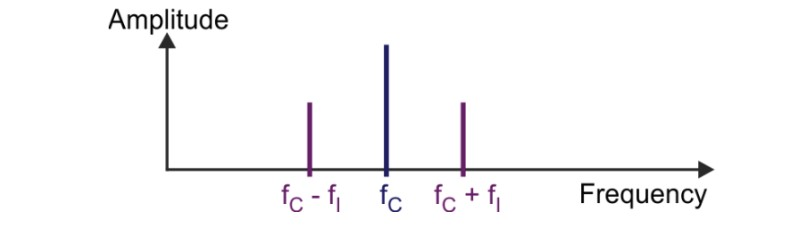
\includegraphics[width=0.45\textwidth]{sineFreqSpec.jpg}
\subsubsection{Range Of Frequencies}
Real signals will be complex waves made up of a range of frequencies. These can be shown on frequency spectrum graphs like so:\\
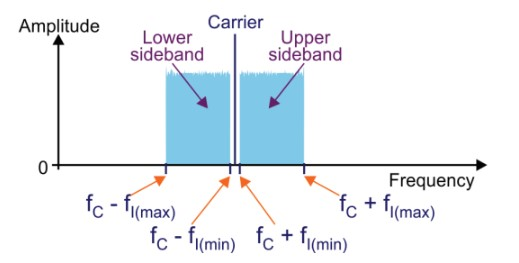
\includegraphics[width=0.45\textwidth]{rangeFreqSpec.jpg}\\
However, the gap between the carrier frequency and the side bands is generally so small that it isn't shown - resulting in a diagram like this:\\
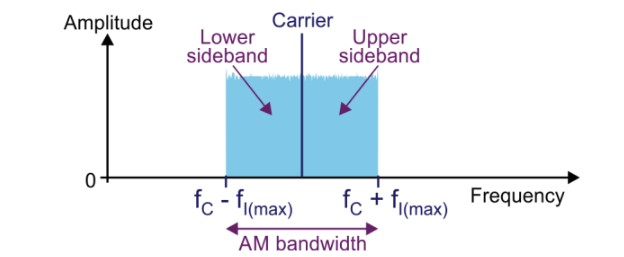
\includegraphics[width=0.45\textwidth]{amBandwidth.jpg}
\subsection{Frequency Allocation (FDM)}
In UK radio broadcasting, each station is bandwidth limited to $5KHz$ therefore the AM bandwidth is $10KHz$ (this includes a $1KHz$ guard band).\\
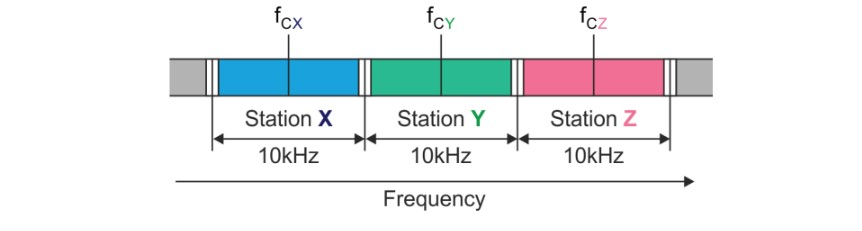
\includegraphics[width=0.45\textwidth]{fdm.jpg}\\
The number of available channels can be calculated using the following equation:\\
$\displaystyle N_{CH} = \frac{\mathrm{Available\ Bandwidth}}{\mathrm{Channel\ Bandwidth}}$
\subsection{Depth Of Modulation}
This is how much the carrier wave is affected by the information wave. If the information signal is greater than the carrier signal ($A_i>A_c$), overmodulation occurs, this gives distortion. \\
$\displaystyle \mathrm{Depth\ Of\ Modulation} = m = \frac{A_i}{A-c}\times 100$\\
$\displaystyle m=\frac{V_{max} - V_{min}}{V_{max} + V_{min}} \times 100$\\
Overmodulation would give $m>100$, generally you shouldn't exceed $80\%$ to leave a safety margin.

\section{FM Radio}
\textit{Frequency Modulated} radio sounds better than AM radio. It is broadcast in the very high frequency range and the amplitude of the wave stays the same, the frequency changes.\\
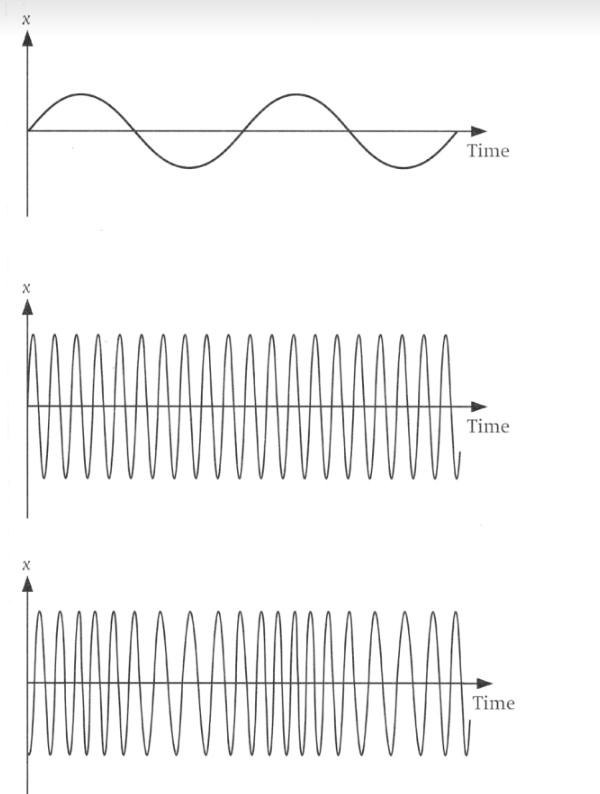
\includegraphics[width=0.45\textwidth]{fmSignal.jpg}\\
The amplitude of the carrier wave changes the frequency of the carrier. If $A=0$, frequency is unchanged. If $A>0$, frequency increases (max. frequency at max. amplitude). If $A<0$, frequency decreases (min. frequency at min. amplitude). 
\subsection{Frequency Deviation}
This is the maximum change in frequency from the carrier's base value $f_c$ which is given the symbol $\Delta f_c$. 
\subsection{Modulation Index}
This describes how modulated the signal is.\\
$\displaystyle \mathrm{Modulation\ Index} = \beta = \frac{\Delta f_c}{f_i}$
\subsection{Frequency Spectrum}
Frequency Modulated signals have infinite sidebands, but some are small enough to ignore. We just care about the 'significant' sidebands. The number of sidebands can be calculated using the following formula: $No = 2(1+\beta)$.\\
In the first graph, $\beta < 1$, the second $\beta = 1$ and the third $\beta = 3$.
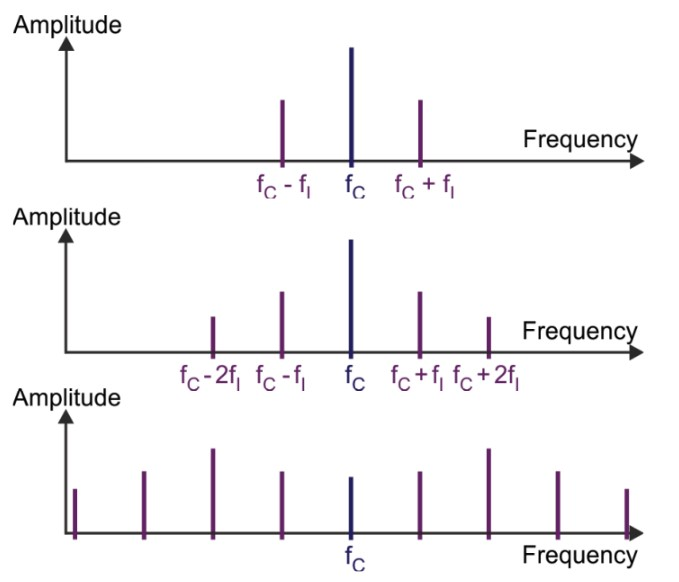
\includegraphics[width=0.45\textwidth]{fmSidebands.jpg}\\
If $\beta < 1$ the signal is said to be narrow band whereas if $\beta >1$ the signal is said to be wideband. 
\subsection{Bandwidth}
FM bandwidth = $2(f_i + \Delta f_c)$
\subsection{Important To Note}
FM Signals are at a constant power because amplitude is always the same and frequency changes are symmetrical. In wideband FM, all the information is in the side bands, therefore the size of the carrier doesn't matter (this is why it can be so small). FM is more efficient than AM.


\end{document}